% Phase 3 (Andrés): Part 1 c, d, e. Every number here comes from src/combinatorics.py (python -m src.combinatorics).
\subsection{Macrostate distribution in log space}
The multiplicity $\Omega(N,k)=\binom{N}{k}=N!/[k!\,(N-k)!]$ grows like $2^N$, so it is computed through its logarithm with the log-Gamma function ($\Gamma(n+1)=n!$, \texttt{math.lgamma}):
\begin{equation}
\ln\Omega(N,k)=\ln\Gamma(N+1)-\ln\Gamma(k+1)-\ln\Gamma(N-k+1).
\end{equation}
\texttt{ln\_omega(N, k)} implements it and \texttt{ln\_omega\_array(N)} evaluates every $k=0\dots N$ at once with \texttt{scipy.special.gammaln}. The tests check $e^{\ln\Omega}$ against the exact integer \texttt{math.comb(N, k)} for all $k$ and $N\le100$ (relative difference below $10^{-11}$), the symmetry $\Omega(N,k)=\Omega(N,N-k)$ and the edges $\Omega(N,0)=\Omega(N,N)=1$, $\Omega(N,1)=N$.

\paragraph{(c) $N=20,50,80,100$.} Figure~\ref{fig:distribution} shows $\Omega(N,k)$ for the four sizes on a logarithmic axis, which is needed because the peaks span 24 orders of magnitude (Table~\ref{tab:peaks}). Each curve is symmetric about $k=N/2$, where the most probable macrostate sits, and falls to $\Omega=1$ at the ordered states $k=0$ and $k=N$. The values are exact integers, so they carry no uncertainty; the log-Gamma route reproduces them to a relative $10^{-11}$. Near the peak each curve is a Gaussian of width $\sigma=\sqrt N/2$: in absolute terms the peak widens with $N$, but relative to the system size it narrows as $\sigma/N=1/(2\sqrt N)$.

\begin{figure}[htbp]\centering
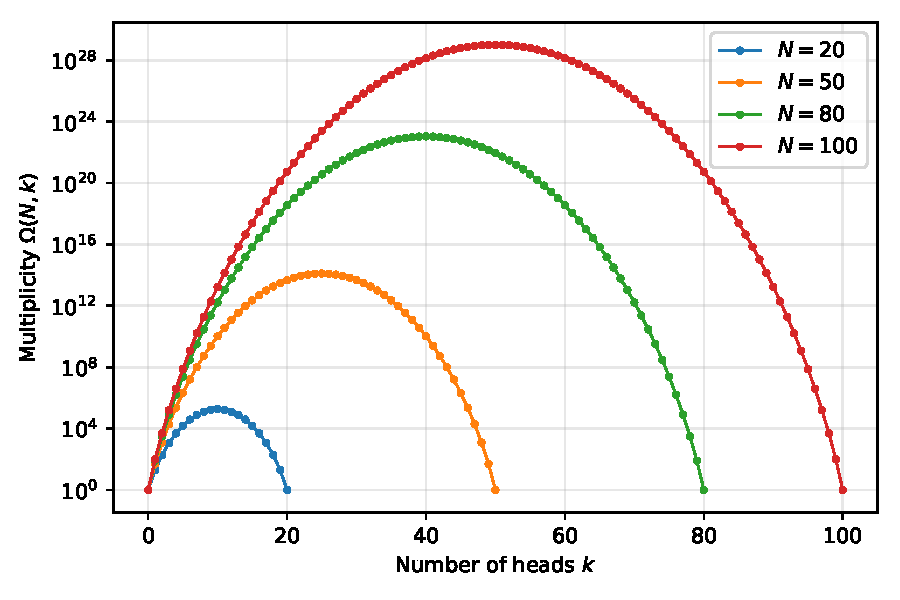
\includegraphics[width=0.75\textwidth]{figures/macrostate_distribution.pdf}
\caption{Number of microstates $\Omega(N,k)$ of each macrostate $k$ (number of heads) for $N=20,50,80,100$ coins, logarithmic vertical axis.}\label{fig:distribution}
\end{figure}

\begin{table}[htbp]\centering\small
\caption{Most probable macrostate $k=N/2$ for each $N$ and the width of the distribution.}\label{tab:peaks}
\begin{tabular}{@{}rrrrr@{}}
\toprule
$N$ & $\Omega(N,N/2)$ & $\ln\Omega(N,N/2)$ & $\sigma=\sqrt N/2$ & $\sigma/N$ \\
\midrule
20 & $1.847560\times10^{5}$ & 12.1268 & 2.24 & 0.112 \\
50 & $1.264106\times10^{14}$ & 32.4706 & 3.54 & 0.071 \\
80 & $1.075072\times10^{23}$ & 53.0318 & 4.47 & 0.056 \\
100 & $1.008913\times10^{29}$ & 66.7838 & 5.00 & 0.050 \\
\bottomrule
\end{tabular}
\end{table}

\paragraph{(d) Largest practical $N$.} Three successive limits were measured on an Apple M4 Max laptop with 48\,GB of RAM:
\begin{itemize}
\item \textbf{Floating-point range (the limit for $\Omega$ itself).} A float64 holds at most $1.8\times10^{308}=e^{709.78}$. The peak $\Omega(N,N/2)$ is the first value to exceed it: \texttt{largest\_float\_N()} gives $N_{\max}=1029$, since $\ln\Omega(1030,515)=710.25$ (checked in the tests: \texttt{float(math.comb(1030, 515))} raises \texttt{OverflowError}). For the same reason $2^N$ overflows at $N=1024$, so probabilities $\Omega/2^N$ must also be formed in log space. Plotting $\Omega$ directly is therefore limited to $N\le1029$; beyond that only $\ln\Omega$ can be plotted.
\item \textbf{Exact integers.} \texttt{math.comb} never overflows (Python integers are arbitrary-precision), but $\Omega(N,N/2)$ has $\approx0.3N$ digits and the arithmetic slows down accordingly. A whole row $k=0\dots N$ took $0.66$\,s for $N=5000$, $4.4$\,s for $N=10^4$ and $30.6$\,s for $N=2\times10^4$, i.e.\ time $\propto N^{2.8}$, which reaches 5 minutes at $N\approx4.5\times10^4$.
\item \textbf{Log space.} $\ln\Omega\approx N\ln2$ never overflows, and a whole row costs about $11$\,ns and $32$\,B per point ($1.1$\,s and $3.2$\,GB for $N=10^8$), so memory caps a full row at $N\approx1.5\times10^9$. Precision then takes over: $\ln\Omega$ is a difference of three numbers of size $\approx N\ln N$, so its absolute error is about one unit in the last place of $\ln\Gamma(N+1)$. Compared with the Stirling/Gaussian form, the error is $2\times10^{-7}$ at $N=10^8$, $2\times10^{-3}$ at $10^{12}$, $0.2$ at $10^{14}$ (so $\Omega$ is uncertain by $\approx20\%$) and $4$ at $10^{15}$ (a factor $e^4$). Past $2^{53}\approx9\times10^{15}$, $k$ itself cannot be stored exactly in a float.
\end{itemize}
In practice, \textbf{the limiting factor is the finite range and precision of floating-point numbers}: $\Omega$ can be computed and plotted up to $N=1029$, and $\ln\Omega$ up to $N\sim10^{13}$, where its error is still below $0.01$. A plot is a weaker constraint than it seems: for large $N$ only the $\sim\sqrt N$ values of $k$ around $N/2$ are visible, so a curve with $10^8$ points carries no more information than one with a thousand.

\paragraph{(e) Scaling to $N\sim10^{23}$.} By the de~Moivre--Laplace theorem, the binomial distribution tends to a Gaussian. Using Stirling's formula, $\ln n!\simeq n\ln n-n+\tfrac12\ln(2\pi n)$, around the peak:
\begin{gather}
\ln\Omega(N,k)\simeq N\ln2+\tfrac12\ln\frac{2}{\pi N}-\frac{2\,(k-N/2)^2}{N},\\
\Omega(N,k)\simeq 2^N\sqrt{\frac{2}{\pi N}}\;e^{-(k-N/2)^2/2\sigma^2},\qquad \sigma=\frac{\sqrt N}{2}.
\end{gather}
This form (\texttt{gaussian\_ln\_omega}) already differs from the exact value at the peak by only $1/(4N)$ in $\ln\Omega$: $0.0125$ for $N=20$ ($1.3\,\%$ in $\Omega$) and $0.0025$ for $N=100$. For $N=10^{23}$:
\begin{itemize}
\item the peak sits at $k=5\times10^{22}$ with $\ln\Omega_{\max}\simeq N\ln2=6.93\times10^{22}$, i.e.\ $\Omega_{\max}\approx10^{3.01\times10^{22}}$, and contains essentially all $2^N$ microstates;
\item the width is $\sigma=\sqrt N/2=1.6\times10^{11}$ coins, enormous in absolute terms but only $\sigma/N=1.6\times10^{-12}$ of the system: on a plot against $k/N$ the distribution is a Dirac delta at $1/2$;
\item a macroscopic deviation is not merely unlikely but impossible in practice: a relative imbalance of one part per million, $k=\tfrac N2(1\pm10^{-6})$, is suppressed by a factor $e^{-2(k-N/2)^2/N}=e^{-5\times10^{10}}\approx10^{-2.2\times10^{10}}$.
\end{itemize}
Physically, this is why thermodynamics works: the macroscopic state (here the fraction of heads, $1/2$) is sharp, fluctuations scale as $1/\sqrt N$ and become unmeasurable, and the entropy $S=k_B\ln\Omega_{\max}\simeq Nk_B\ln2$ is extensive. Computationally, neither $\Omega$ nor even \texttt{lgamma} can be used at this size: one unit in the last place of $\ln\Gamma(10^{23}+1)$ is $\approx10^9$, so the large-$N$ results must come from the analytic Stirling/Gaussian expressions above (developed further in Part~2\,k).
